% !TeX program = xelatex
% !BIB program = biber
\documentclass[light]{lutbeamer}

\usepackage{pgfpages}
\usepackage{ragged2e}
\usepackage{booktabs}
\usepackage{amssymb}
\usepackage{fontawesome5}
\usepackage{tikz}
\usepackage{pgfplots}
\pgfplotsset{compat=1.18}
\addbibresource{references.bib}

% ===================================================================
% METADATA
% ===================================================================
\setdepartment{OSTIM Teknik Üniversitesi}
\institute{}
\author[Mühendislik Fakültesi]{\\
Prof.~Dr.~Yalçın ATA \\
Prof.~Dr.~Arif DEMİR \\
Dr.~Öğr.~Üyesi~Muhammed ELMNEFİ \\
Dr.~Öğr.~Üyesi~Haydar KILIÇ \\
Dr.~Öğr.~Üyesi~Emel GÜVEN \\
Dr.~Öğr.~Üyesi~Ufuk ASIL \\
Öğr.~Gör.~Sema ÇİFTÇİ
}
\title{MATH 204 -- Olasılık ve İstatistik}
\subtitle{Hafta 9: Ayrık Olasılık Dağılımları}
\date{2025--2026 Bahar Dönemi}

% ===================================================================
% OTOMATİK İÇİNDEKİLER
% ===================================================================
\setcounter{tocdepth}{2}

\AtBeginSection[]{
  \begin{frame}{Sunum Planı}
    \scriptsize
    \begin{columns}[T]
      \begin{column}{0.48\textwidth}
        \tableofcontents[sections={1-3}, currentsection]
      \end{column}
      \begin{column}{0.48\textwidth}
        \tableofcontents[sections={4-10}, currentsection]
      \end{column}
    \end{columns}
  \end{frame}
}

\begin{document}

\setbeamertemplate{navigation symbols}{}
\setbeamertemplate{footline}{
  \begin{beamercolorbox}[wd=\paperwidth, ht=10pt, dp=1pt]{footline}
    \usebeamerfont{footline}
    \begin{tikzpicture}[remember picture,overlay]
      \node[anchor=south west, xshift=10mm, yshift=.4mm]
      at (current page.south west)
      {\insertshortauthor,~\department};
    \end{tikzpicture}
    \begin{tikzpicture}[remember picture,overlay]
      \node[anchor=south east, xshift=-5mm, yshift=0.5mm]
      at (current page.south east)
      {\insertframenumber \,/\, \inserttotalframenumber};
    \end{tikzpicture}
  \end{beamercolorbox}
}

% ===================================================================
% KAPAK
% ===================================================================
\begin{frame}<article:0>[plain,noframenumbering]
  \begin{tikzpicture}[remember picture,overlay]
    \node[anchor=center, at=(current page.center), inner sep=0pt] {
      \includegraphics[width=\paperwidth, height=\paperheight]{logos/background_figure.jpg}
    };
  \end{tikzpicture}
\end{frame}

{
  \setbeamertemplate{footline}{
    \begin{beamercolorbox}[wd=\paperwidth, ht=10pt, dp=1pt]{footline}
      \usebeamerfont{footline}
      \begin{tikzpicture}[remember picture,overlay]
        \node[anchor=south west, xshift=10mm, yshift=.4mm, align=left]
        at (current page.south west)
        {\tiny Bu şablon OTU Yazılım Mühendisliği tarafından hazırlanmış olup \href{https://github.com/ufukasia/Ostim-Teknik--niversitesi-Yaz-l-m-M-hendisli-i---Lutbeamer-egitim-i-eri-i-haz-rlama-}{buradan} güncel haline ulaşabilirsiniz.};
      \end{tikzpicture}
      \begin{tikzpicture}[remember picture,overlay]
        \node[anchor=south east, xshift=-5mm, yshift=0.5mm]
        at (current page.south east)
        {\insertframenumber \,/\, \inserttotalframenumber};
      \end{tikzpicture}
    \end{beamercolorbox}
  }
  \setbeamerfont{title}{size=\large}
  \setbeamerfont{author}{size=\scriptsize}
  \setbeamerfont{subtitle}{size=\small}
  \setbeamerfont{date}{size=\footnotesize}
  \maketitle{}
}

\begin{frame}{İçindekiler}
  \scriptsize
  \begin{columns}[T]
    \begin{column}{0.48\textwidth}
      \tableofcontents[sections={1-3}]
    \end{column}
    \begin{column}{0.48\textwidth}
      \tableofcontents[sections={4-10}]
    \end{column}
  \end{columns}
\end{frame}

% ===================================================================
% SECTION 1
% ===================================================================
\section{Vizeden Bu Haftaya ve Ayrık Uniform (Bölüm 5.1)}
\subsection{Hatırlatma ve Köprü}

\begin{frame}{Vizeden Bu Haftaya: Hangi Dili Hazır Getiriyoruz?}
    \small
    \begin{block}{Önceki haftalardan elimizde olan yapı}
        \[
        P(X=x)=f(x), \qquad \sum_x f(x)=1,
        \]
        \[
        E(X)=\sum_x x f(x), \qquad \mathrm{Var}(X)=E(X^2)-[E(X)]^2.
        \]
    \end{block}

    \begin{itemize}
        \item Hafta 4'te rastgele değişkeni ve PMF dilini kurduk.
        \item Sonraki haftalarda beklenen değer, varyans ve standart sapma ile dağılımları okumayı öğrendik.
        \item Vizeden sonra artık soru şudur: \textbf{Verilen sayım problemi için hangi ayrık dağılım ailesi uygundur?}
    \end{itemize}

    \begin{exampleblock}{Bu haftanın yönü}
        Tek tek PMF tablosu yazmak yerine, aynı davranışı paylaşan problemleri \textbf{hazır dağılım aileleri} ile modelleyeceğiz.
    \end{exampleblock}
\end{frame}

\begin{frame}{Kavram Haritası: Ayrık Dağılım Aileleri}
    \centering
    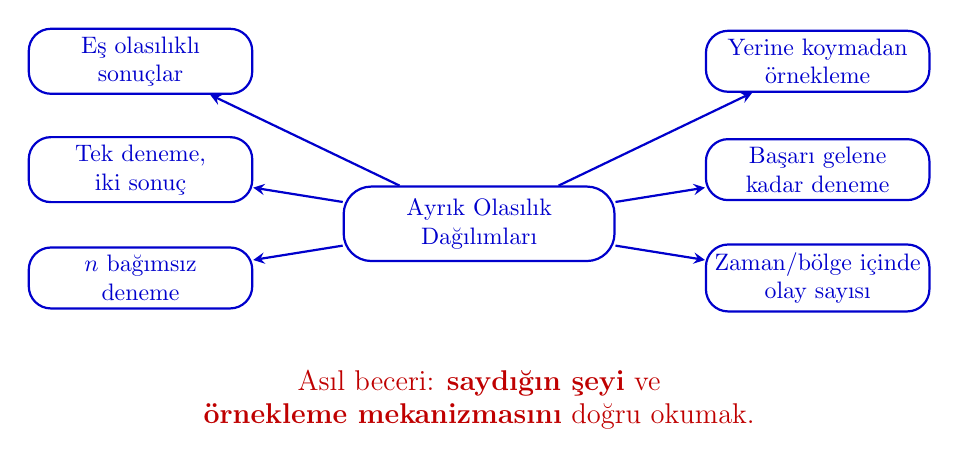
\begin{tikzpicture}[>=stealth, thick, scale=0.86, transform shape]
        \colorlet{myblue}{blue!80!black}
        \colorlet{myred}{red!75!black}

        \node[draw=myblue, rounded corners=10pt, minimum width=4.0cm, minimum height=1.1cm, text=myblue, align=center] (root) at (0,0) {Ayrık Olasılık\\Dağılımları};

        \node[draw=myblue, rounded corners=8pt, minimum width=3.3cm, minimum height=0.9cm, text=myblue, align=center] (uniform) at (-5,2.4) {Eş olasılıklı\\sonuçlar};
        \node[draw=myblue, rounded corners=8pt, minimum width=3.3cm, minimum height=0.9cm, text=myblue, align=center] (bern) at (-5,0.8) {Tek deneme,\\iki sonuç};
        \node[draw=myblue, rounded corners=8pt, minimum width=3.3cm, minimum height=0.9cm, text=myblue, align=center] (binom) at (-5,-0.8) {$n$ bağımsız\\deneme};
        \node[draw=myblue, rounded corners=8pt, minimum width=3.3cm, minimum height=0.9cm, text=myblue, align=center] (hyper) at (5,2.4) {Yerine koymadan\\örnekleme};
        \node[draw=myblue, rounded corners=8pt, minimum width=3.3cm, minimum height=0.9cm, text=myblue, align=center] (geom) at (5,0.8) {Başarı gelene\\kadar deneme};
        \node[draw=myblue, rounded corners=8pt, minimum width=3.3cm, minimum height=0.9cm, text=myblue, align=center] (pois) at (5,-0.8) {Zaman/bölge içinde\\olay sayısı};

        \draw[->, myblue] (root) -- (uniform);
        \draw[->, myblue] (root) -- (bern);
        \draw[->, myblue] (root) -- (binom);
        \draw[->, myblue] (root) -- (hyper);
        \draw[->, myblue] (root) -- (geom);
        \draw[->, myblue] (root) -- (pois);

        \node[text=myred, font=\large, align=center] at (0,-2.6) {Asıl beceri: \textbf{saydığın şeyi} ve\\ \textbf{örnekleme mekanizmasını} doğru okumak.};
    \end{tikzpicture}
\end{frame}

\subsection{Ayrık Uniform (Bölüm 5.1)}

\begin{frame}{Isınma: Ayrık Uniform (Bölüm 5.1)}
    \scriptsize
    \begin{columns}[T]
        \begin{column}{0.48\textwidth}
            \begin{block}{Ayrık uniform dağılım}
                Sonuç kümesindeki tüm değerler \textbf{eş olasılıklı} ise ayrık uniform dağılımdan söz ederiz.
                \[
                P(X=x_i)=\frac{1}{k}, \qquad i=1,\dots,k.
                \]
                En klasik örnekler: adil zar, numaralı etiket çekimi, eş olasılıklı kart seçimi.
            \end{block}

            \begin{exampleblock}{Özel durum}
                Eğer
                \[
                X \in \{1,2,\dots,m\}
                \]
                ise
                \[
                E(X)=\frac{m+1}{2}, \qquad \mathrm{Var}(X)=\frac{m^2-1}{12}.
                \]
            \end{exampleblock}
        \end{column}
        \begin{column}{0.48\textwidth}
            \begin{block}{Zar örneği}
                \[
                P(X=x)=\frac{1}{6}, \qquad x=1,2,3,4,5,6.
                \]
                Bu durumda
                \[
                E(X)=3.5, \qquad \mathrm{Var}(X)=\frac{35}{12}.
                \]
            \end{block}

            \begin{exampleblock}{Köprü}
                Buradaki ana ölçüt, \textbf{tüm sonuçların eş olasılıklı} olmasıdır.
                Bir sonraki frame'de bunu Bernoulli ile karşılaştıracağız.
            \end{exampleblock}
        \end{column}
    \end{columns}
\end{frame}

\begin{frame}{Mini Soru 0: Ayrık Uniformda Sayısal Okuma}
    \scriptsize
    \begin{columns}[T,onlytextwidth]
        \begin{column}{0.48\textwidth}
            \begin{block}{Soru}
                \(1\)'den \(10\)'a numaralı, eş olasılıklı test çiplerinden biri seçiliyor.
                \(X\), seçilen çip numarası olsun.
                \begin{enumerate}
                    \item[(a)] Seçilen çipin 7 numaralı olma olasılığı \(P(X=7)\) nedir?
                    \item[(b)] Seçilen çip numarasının beklenen değeri \(E(X)\) nedir?
                    \item[(c)] Seçilen çip numarasının varyansı \(\mathrm{Var}(X)\) nedir?
                \end{enumerate}
            \end{block}
        \end{column}
        \begin{column}{0.48\textwidth}
            \begin{exampleblock}{Çözüm}
                Her sonuç eş olasılıklı olduğu için
                \[
                P(X=7)=\frac{1}{10}=0.10.
                \]
                Ayrıca
                \[
                E(X)=\frac{10+1}{2}=5.5,
                \]
                \[
                \mathrm{Var}(X)=\frac{10^2-1}{12}=8.25.
                \]
                Yani model hem nokta olasılığını hem de merkezi doğrudan verir.
            \end{exampleblock}
        \end{column}
    \end{columns}
\end{frame}

\begin{frame}{Mini Quiz: Bernoulli mi, Ayrık Uniform mu?}
    \small
    \begin{columns}[T]
        \begin{column}{0.48\textwidth}
            \begin{block}{Bernoulli}
                \begin{itemize}
                    \item değer kümesi: \(\{0,1\}\) (örn. geçti=\(1\), kaldı=\(0\))
                    \item yalnızca iki kategori vardır (örn. bozuk veya sağlam)
                    \item tek parametre: \(p\) (örn. sınavdan geçme olasılığı \(0.90\))
                    \item ``başarı sayısı'' diline çok uygundur
                \end{itemize}
            \end{block}
        \end{column}
        \begin{column}{0.48\textwidth}
            \begin{block}{Ayrık uniform}
                \begin{itemize}
                    \item değer kümesi: \(k\) adet ayrık değer (örn. \(1,2,\dots,10\))
                    \item tüm değerler eş olasılıklıdır (örn. her etikete \(1/10\))
                    \item parametre çoğunlukla değer kümesidir (örn. \(k=10\))
                    \item numara, etiket, kart seçimi gibi yapılara uygundur
                \end{itemize}
            \end{block}
        \end{column}
    \end{columns}

    \begin{exampleblock}{Hızlı karar soruları}
        \begin{enumerate}
            \item Tek bir sensörün geçti/kaldı sonucu: \textbf{Bernoulli}
            \item \(8\) etiketten birinin eş olasılıkla seçilmesi: \textbf{ayrık uniform}
        \end{enumerate}
    \end{exampleblock}

    \begin{alertblock}{Dikkat}
        Bernoulli ile iki noktalı ayrık uniform yalnızca \(p=0.5\) olduğunda çakışır; genel durumda aynı model değildir.
    \end{alertblock}
\end{frame}

% ===================================================================
% SECTION 2
% ===================================================================
\section{Bernoulli Süreci ve Binom Dağılımı (Bölüm 5.2)}
\subsection{Bernoulli Süreci}

\begin{frame}{Bernoulli Süreci Nedir?}
    \small
    Bir deney aşağıdaki dört özelliği taşıyorsa \textbf{Bernoulli süreci} olarak okunur:
    \begin{enumerate}
        \item Deney tekrarlı yapılır (örn. üretim bandından \(12\) adet sensörün tek tek test edilmesi).
        \item Her deneme yalnızca \textbf{başarı} veya \textbf{başarısızlık} üretir (örn. sensörün testten geçmesi veya kalması).
        \item Başarı olasılığı her denemede sabittir: \(p\) (örn. her sensör için testten geçme olasılığının hep \(0.90\) kalması).
        \item Denemeler birbirinden bağımsızdır (örn. önceki sensörün testten kalması, sonrakinin bozuk olma ihtimalini etkilemez).
    \end{enumerate}

    \begin{exampleblock}{Mühendislik okuması}
        Her kart için ``kusurlu / kusursuz'', her modem için ``bağlandı / bağlanmadı'', her test için ``geçti / kaldı'' dili Bernoulli süreci kurmaya adaydır.
    \end{exampleblock}
\end{frame}

\begin{frame}{Mini Soru 1: Tek Sensörlük Bernoulli Modeli}
    \scriptsize
    \begin{columns}[T,onlytextwidth]
        \begin{column}{0.48\textwidth}
            \begin{block}{Soru}
                Bir sensörün tek denemede kalibrasyonu geçme olasılığı \(0.80\) olsun.
                \[
                X=
                \begin{cases}
                1, & \text{geçerse},\\
                0, & \text{kalırsa}.
                \end{cases}
                \]
                \(P(X=1)\), \(E(X)\) ve \(\mathrm{Var}(X)\) nedir?
            \end{block}
        \end{column}
        \begin{column}{0.48\textwidth}
            \begin{exampleblock}{Çözüm}
                Bu tek denemelik bir Bernoulli modelidir:
                \[
                X\sim \mathrm{Bern}(0.80).
                \]
                Dolayısıyla
                \[
                P(X=1)=0.80,
                \]
                \[
                E(X)=0.80,\qquad \mathrm{Var}(X)=0.80(0.20)=0.16.
                \]
                Tek denemede sayı dili kurulduğunda, ortalama ve varyans da hemen okunur.
            \end{exampleblock}
        \end{column}
    \end{columns}
\end{frame}

\begin{frame}{Neden Her Soruda Sıfırdan Olasılık Tablosu (PMF) Kurmuyoruz?}
    \small
    \begin{columns}[T]
        \begin{column}{0.48\textwidth}
            \begin{block}{Eski Yöntemimizin Zorluğu (Hafta 4)}
                Önceki haftalarda bir problemi çözerken tüm ihtimalleri inceliyor ve tek tek hesaplayarak bir olasılık tablosu (PMF - Olasılık Kütle Fonksiyonu) çiziyorduk. 
            \end{block}

            \begin{block}{Fakat Hikayeler Hep Tekrar Eder!}
                \begin{itemize}
                    \item Banttaki \(10\) üründe arızalı parça sayısını bulmak
                    \item Çekilen \(5\) karttaki kırmızı kart sayısını bulmak
                \end{itemize}
                Dikkat ederseniz bu iki problem tamamen \textbf{aynı iskelete} sahiptir. Her yeni soruda amele gibi sıfırdan tablo kurmak büyük bir vakit kaybıdır.
            \end{block}
        \end{column}
        \begin{column}{0.48\textwidth}
            \begin{exampleblock}{Çözüm: Hazır Dağılım Aileleri}
                Birbirine benzeyen problemleri gruplayıp onlara özel hazır formüller (örn. Binom, Poisson) oluştururuz. Bunun müthiş faydaları vardır:
                \begin{itemize}
                    \item Uzun tablolar çizmek yerine \textbf{tek bir sabit formülle} doğrudan sonuca gitmek.
                    \item Beklenen değer ve varyansı hesaplamaya uğraşmadan \textbf{formülden okuyabilmek}.
                    \item Problemin şifresini anında çözmek.
                \end{itemize}
            \end{exampleblock}

            \vspace{0.2cm}
            \centering
            \textit{Ana Fikir: Uzun hesaplara girişmeden önce şunu sorarız: ``Bu olay hangi hazır kalıba (dağılıma) uyuyor?''}
        \end{column}
    \end{columns}
\end{frame}

\begin{frame}{Bernoulli Değişkeni: Değişken ve Dağılım Farkı}
    \small
    \textbf{Bernoulli Dağılımı}, olayın olasılığının bizzat kendisidir (örn. geçme olasılığının \(0.80\) olması). 
    
    \textbf{Bernoulli Değişkeni} (\(X\)) ise, ``testi geçti'' veya ``bozuk'' gibi \textbf{sözel olan bir sonucu}, matematikte kullanabilmek için basit bir puan sistemine (\(1\) veya \(0\)) dönüştüren araçtır.

    \begin{block}{Durumu Sayıya Çevirmek (Puan Verme Sistemi)}
        \[
        X=
        \begin{cases}
        1, & \text{İstediğimiz durum gerçekleştiyse (\textbf{Başarı})},\\
        0, & \text{İstediğimiz durum olmadıysa (\textbf{Başarısızlık})}.
        \end{cases}
        \]
    \end{block}

    \begin{exampleblock}{Bu Değişken (\(X\)) Bizi Binom'a Nasıl Götürecek?}
        Diyelim ki banttan peş peşe \(5\) adet sensör aldınız ve test ettiniz.
        \begin{itemize}
            \item Sensörlerin ürettiği değişkenler (\(X\)): Geçti~(\(1\)), Kaldı~(\(0\)), Geçti~(\(1\)), Geçti~(\(1\)), Kaldı~(\(0\))
            \item Matematikte bu bağımsız skorları topladığımızda: \(1+0+1+1+0 = 3\)
            \item \textbf{Ana Fikir:} Bireysel Bernoulli değişkenlerini (\(X\)) yan yana toplayarak saniyeler içinde ``toplam başarı sayısını'' bulmuş olduk. İşte tekli olayların yan yana toplanıp birleştiği bu yeni ve büyük yapıya \textbf{Binom Dağılımı} diyoruz!
        \end{itemize}
    \end{exampleblock}
\end{frame}

\subsection{Binom Dağılımı}

\begin{frame}{Binom Dağılımı: Saydığımız Başarı Sayısı}
    \scriptsize
    \begin{block}{Tanım}
        \(n\) bağımsız Bernoulli denemesinde başarı olasılığı \(p\) ise,
        başarı sayısı \(X\) için
        \[
        X \sim \mathrm{Bin}(n,p)
        \]
        yazılır.
    \end{block}

    \begin{itemize}
        \item \(X\), \textbf{kaç başarı geldiğini} sayar.
        \item Değer kümesi
        \[
        X=\{0,1,2,\dots,n\}
        \]
        olur.
        \item Her denemede olasılık sabit değilse veya bağımsızlık bozulursa binom modeli zayıflar.
    \end{itemize}

    \begin{block}{Ana fikir}
        \textbf{Bernoulli dağılımı, binom dağılımının \(n=1\) özel halidir.}
        Binom, bu tek denemelik 0--1 yapının \(n\) denemede başarı sayısını sayan sürümüdür.
    \end{block}
\end{frame}

\begin{frame}{Binom Sezgisi: Hileli Para Örneği}
    \footnotesize
    Hileli bir para olsun:
    \(\textcolor{blue}{p(\text{tura}) = 0{,}6}\),
    \(\textcolor{red}{p(\text{yazı}) = 0{,}4}\).
    Bu para \(5\) kez atılsın. \textbf{İki kez yazı gelme olasılığı nedir?}

    \textbf{Adım 1: Tek bir sıra.}
    \(\textcolor{red}{Y},\textcolor{red}{Y},\textcolor{blue}{T},\textcolor{blue}{T},\textcolor{blue}{T}\) gibi belirli bir sıra için olasılık
    \(\textcolor{red}{(0{,}4)^{2}}\textcolor{blue}{(0{,}6)^{3}}\)'tür.

    \textbf{Adım 2: Kaç farklı sıra var?}
    Yazılar her zaman ilk iki denemede gelmek zorunda değil; örn.
    \(\textcolor{red}{Y},\textcolor{red}{Y},\textcolor{blue}{T},\textcolor{blue}{T},\textcolor{blue}{T}\)\qquad
    \(\textcolor{blue}{T},\textcolor{red}{Y},\textcolor{red}{Y},\textcolor{blue}{T},\textcolor{blue}{T}\)\qquad
    \(\textcolor{red}{Y},\textcolor{blue}{T},\textcolor{red}{Y},\textcolor{blue}{T},\textcolor{blue}{T}\), \dots
    Bu yüzden \(\binom{5}{2} = 10\) farklı dizilim vardır.

    \textbf{Adım 3: Formülü bir araya getir.}
    \[
    P(Y=2)=\binom{5}{2}\textcolor{red}{(0{,}4)^{2}}\textcolor{blue}{(0{,}6)^{3}}=10\cdot 0{,}16\cdot 0{,}216=0{,}2304
    \]

    Genel formülle karşılaştır:
    \[
    b(x;\,n,p) = \binom{n}{x}\,p^{x}\,(1-p)^{n-x}
    \]
    Burada \(n=5\), \(x=2\), \(\textcolor{red}{p=0{,}4}\) (yazı = ``başarı'').
\end{frame}

\begin{frame}{Binom Formülü Neden Böyle Görünür?}
    \scriptsize
    Tam \(x\) başarı gelmesi için iki şey gerekir:
    \begin{enumerate}
        \item Belirli bir sıranın olasılığı: \(p^x(1-p)^{n-x}\)
        \item Bu sıranın kaç farklı şekilde oluşabileceği: \(\binom{n}{x}\)
    \end{enumerate}

    \begin{block}{Binom olasılık fonksiyonu}
        \[
        b(x;n,p)=\binom{n}{x}p^x(1-p)^{n-x},
        \qquad x=0,1,\dots,n.
        \]
    \end{block}

    \begin{block}{Okuma}
        \(\binom{n}{x}\) düzen sayısını, \(p^x(1-p)^{n-x}\) ise her düzenin ağırlığını taşır.
    \end{block}
\end{frame}

\begin{frame}{Örnek 1: Şok Testini Geçen Parça Sayısı}
    \small
    Bir bileşenin şok testini geçme olasılığı \(p=0.75\) olsun. Sıradaki \(4\) bileşenden tam(yalnız) \(2\) tanesinin testi geçme olasılığı nedir?

    \vspace{0.2cm}
    \begin{block}{Model}
        \[
        X \sim \mathrm{Bin}(4,0.75), \qquad P(X=2)=\binom{4}{2}(0.75)^2(0.25)^2.
        \]
    \end{block}

    \[
    \binom{4}{2}=6,\qquad (0.75)^2=0.5625,\qquad (0.25)^2=0.0625
    \]
    \[
    P(X=2)=6(0.5625)(0.0625)=0.2109.
    \]

    \begin{exampleblock}{Yorum}
        Tam iki başarılı bileşen görme olasılığı yaklaşık \(\%21.1\)'dir.
    \end{exampleblock}
\end{frame}

\begin{frame}{Örnek 2: Kuyu Örneklemesinde Tam 3 Kirli Kuyu}
    \small
    Bir bölgede kuyuların \(\%30\)'unun kirli olduğu biliniyor. Rastgele seçilen \(10\) kuyudan tam \(3\)'ünün kirli olma olasılığını bulun.

    \vspace{0.2cm}
    \[
    X \sim \mathrm{Bin}(10,0.30)
    \]
    \[
    P(X=3)=\binom{10}{3}(0.30)^3(0.70)^7.
    \]
    \[
    \binom{10}{3}=120,\qquad (0.30)^3=0.027,\qquad (0.70)^7\approx 0.08235
    \]
    \[
    P(X=3)=120(0.027)(0.0823543)\approx 0.2668.
    \]

    \begin{exampleblock}{Mesaj}
        ``Kuyu sayısı sabit, her kuyu için kirli/temiz ayrımı var, oran sabit'' olduğu için binom doğrudur.
    \end{exampleblock}
\end{frame}

\begin{frame}{Örnek 3: Batarya Paketinde Kabul Aralığı}
    \scriptsize
    \begin{columns}[T,onlytextwidth]
        \begin{column}{0.48\textwidth}
            \begin{block}{Soru}
                Bir batarya paketindeki her hücrenin testi geçme olasılığı \(0.40\) olsun.
                Üretimden gelen \(8\) hücrelik bir pakette,
                \textbf{en az \(3\), en fazla \(5\)} hücrenin testi geçmesi
                sevkiyat için yeterli kabul ediliyor.

                Bu paketin kabul edilme olasılığı nedir?
            \end{block}
        \end{column}
        \begin{column}{0.48\textwidth}
            \begin{exampleblock}{Çözüm}
                \[
                X\sim \mathrm{Bin}(8,0.40)
                \]
                İstenen olasılık
                \[
                P(3\le X\le 5)=\sum_{x=3}^{5}\binom{8}{x}(0.40)^x(0.60)^{8-x}.
                \]
                Hesaplanırsa
                \[
                P(3\le X\le 5)\approx 0.6348.
                \]
                Sevkiyat kabul olasılığı yaklaşık \(\%63.5\)'tir.
            \end{exampleblock}
        \end{column}
    \end{columns}
\end{frame}

\begin{frame}{Ortalama ve Varyans: Binomun Merkezi ve Yayılımı}
    \small
    \(X \sim \mathrm{Bin}(n,p)\) için
    \[
    \mu = E(X)=np, \qquad \sigma^2=\mathrm{Var}(X)=np(1-p).
    \]

    \begin{columns}[T]
        \begin{column}{0.48\textwidth}
            \begin{block}{Sezgi}
                \begin{itemize}
                    \item \(np\): beklenen başarı sayısı
                    \item \(1-p\): başarısızlık payı
                    \item yayılım, hem başarı hem başarısızlık olasılığına bağlı
                \end{itemize}
            \end{block}
        \end{column}
        \begin{column}{0.48\textwidth}
            \begin{exampleblock}{Kısa örnek}
                Eğer \(n=15\) ve \(p=0.4\) ise
                \[
                E(X)=15(0.4)=6,
                \]
                \[
                \mathrm{Var}(X)=15(0.4)(0.6)=3.6.
                \]
            \end{exampleblock}
        \end{column}
    \end{columns}
\end{frame}

\begin{frame}{Binom Sorularında Kontrol Listesi}
    \small
    \begin{enumerate}
        \item Deneme sayısı sabit mi?
        \item Her denemede yalnızca iki sonuç mu var?
        \item Başarı olasılığı sabit mi?
        \item Denemeler bağımsız mı?
        \item Aradığımız şey \textbf{başarı sayısı} mı?
    \end{enumerate}

    \begin{alertblock}{Sık hata}
        ``Örneklem büyüklüğü sabit'' görmek tek başına yetmez. Eğer seçim \textbf{yerine koymadan} yapılıyorsa hipergeometrik düşünmek gerekir.
    \end{alertblock}
\end{frame}

\subsection{Pekiştirme Soruları}

\begin{frame}{Soru 1: Lehim Hattında Kusurlu Kart Sayısı}
    \small
    Bir elektronik kart hattında her kartın kusurlu çıkma olasılığı \(0.08\) olarak modelleniyor ve kartlar bağımsız kabul ediliyor. Rastgele seçilen \(12\) kart için:

    \begin{enumerate}
        \item[(a)] Tam \(2\) kartın kusurlu olma olasılığını bulun.
        \item[(b)] En fazla \(2\) kartın kusurlu olma olasılığını bulun.
    \end{enumerate}

    \begin{block}{İpucu}
        Bu bir \textbf{başarı sayısı} problemidir; burada başarıyı ``kart kusurlu'' diye okuyun.
    \end{block}
\end{frame}

\begin{frame}{Soru 1: Çözüm İçin Durak}
    \color{red!70!black}
    \small
    \[
    X \sim \mathrm{Bin}(12,0.08)
    \]
    Burada başarıyı ``kart kusurlu'' olarak okuyun.
    \begin{itemize}
        \item[(a)] nokta olasılığı: tam \(2\) kusurlu
        \item[(b)] kümülatif olasılık: en fazla \(2\) kusurlu
    \end{itemize}

    \begin{center}
        \textit{Önce modeli ve parametreleri doğrulayın; sayısal hesabı siz tamamlayın.}
    \end{center}
\end{frame}

\begin{frame}{Soru 1: Çözüm}
    \small
    \[
    P(X=2)=\binom{12}{2}(0.08)^2(0.92)^{10}\approx 0.1835.
    \]

    \[
    P(X\le 2)=\sum_{x=0}^{2}\binom{12}{x}(0.08)^x(0.92)^{12-x}\approx 0.9348.
    \]

    \begin{exampleblock}{Yorum}
        Süreç kusur oranı düşük olduğu için \(12\) kart içinde \(2\) veya daha az kusurlu kart görme olasılığı oldukça yüksektir.
    \end{exampleblock}
\end{frame}

\begin{frame}{Soru 2: Bernoulli mi, Binom mu?}
    \small
    Bir sensörün tek denemede kalibrasyonu geçme olasılığı \(0.90\) olsun.
    \begin{enumerate}
        \item[(i)] \(X=1\) geçerse, \(X=0\) kalırsa: \(P(X=1)\), \(E(X)\), \(\mathrm{Var}(X)\)
        \item[(ii)] Aynı tip \(20\) sensörden kalibrasyonu geçenlerin sayısı \(Y\) için uygun dağılım
    \end{enumerate}

    \begin{block}{İpucu}
        (i) tek deneme, (ii) sabit sayıda denemede başarı sayısı.
    \end{block}
\end{frame}

\begin{frame}{Soru 2: Çözüm}
    \small
    \begin{itemize}
        \item[(i)] Tek sensör için \(X\sim \mathrm{Bern}(0.90)\). Bu yüzden
        \[
        P(X=1)=0.90,\qquad E(X)=0.90,\qquad \mathrm{Var}(X)=0.90(0.10)=0.09.
        \]
        \item[(ii)] \(20\) sensörde geçen sayısı için
        \[
        Y\sim \mathrm{Bin}(20,0.90).
        \]
    \end{itemize}

    \begin{block}{Kural}
        \[
        \text{Bernoulli} = \text{Binomun } n=1 \text{ özel hali.}
        \]
    \end{block}
\end{frame}

% ===================================================================
% SECTION 3
% ===================================================================
\section{Çok Kategorili Sayım ve Multinomial Uzantısı (Bölüm 5.2'nin Genellemesi)}
\subsection{Binomun Genişlemesi}

\begin{frame}{İki Sonuç Yetmezse: Multinomial Fikir}
    \small
    Binom dağılımında her denemede yalnızca iki sonuç vardı: başarı veya başarısızlık.

    \vspace{0.2cm}
    Peki her denemede \(k\) farklı sonuç varsa ne olur?

    \begin{itemize}
        \item trafik yönü: kuzey, güney, doğu, batı
        \item kalite sınıfı: A, B, C
        \item ulaşım türü: kara, hava, demir, deniz
    \end{itemize}

    \begin{exampleblock}{Köprü}
        Bu durumda başarı sayısı değil, \textbf{her kategoride kaç gözlem geldiğini} birlikte sayarız.
    \end{exampleblock}
\end{frame}

\begin{frame}{Multinomial Dağılım: Genel Formül}
    \small
    Her denemede \(k\) kategori olsun ve olasılıklar
    \[
    p_1,p_2,\dots,p_k, \qquad p_1+\cdots+p_k=1.
    \]
    \(n\) denemede \(x_1,\dots,x_k\) sayıları gözlenirse
    \[
    x_1+\cdots+x_k=n
    \]
    ve olasılık
    \[
    P(X_1=x_1,\dots,X_k=x_k)=
    \frac{n!}{x_1!\cdots x_k!}p_1^{x_1}\cdots p_k^{x_k}.
    \]

    \begin{block}{Özel durum}
        \(k=2\) olduğunda multinomial, binom dağılımına geri döner.
    \end{block}
\end{frame}

\begin{frame}{Uygulama: Kavşakta Yön Dağılımı}
    \small
    Bir kavşakta gelen araçların yön oranları sırasıyla
    \[
    p_{\text{kuzey}}=0.15,\quad p_{\text{güney}}=0.25,\quad p_{\text{doğu}}=0.60
    \]
    olsun. \(12\) araç içinde \(2\) kuzey, \(3\) güney ve \(7\) doğu yönlü araç görme olasılığı:
    \[
    \frac{12!}{2!3!7!}(0.15)^2(0.25)^3(0.60)^7.
    \]

    \[
    P\approx 0.0779.
    \]

    \begin{exampleblock}{Yorum}
        Burada binom yeterli değildir; çünkü tek başarı kategorisi değil, \textbf{üçlü dağılım profili} önemlidir.
    \end{exampleblock}
\end{frame}

\begin{frame}{Mini Quiz: Binom mu, Multinomial mi?}
    \scriptsize
    \begin{columns}[T]
        \begin{column}{0.48\textwidth}
            \begin{block}{Binom}
                \begin{itemize}
                    \item İki kategori (örn. kusurlu, kusursuz)
                    \item Tek başarı sayısı (örn. toplam kusurlu sayısı)
                    \item Parametreler: \(n,p\) (örn. \(12\) kart, \(p=0.08\))
                \end{itemize}
            \end{block}
        \end{column}
        \begin{column}{0.48\textwidth}
            \begin{block}{Multinomial}
                \begin{itemize}
                    \item Birden çok kategori (örn. A, B, C kalite sınıfları)
                    \item Kategori sayılarının tamamı (örn. kaç adet A, kaç adet B çıktı)
                    \item Parametreler: \(n,p_1,\dots,p_k\) (örn. oran dağılımları)
                \end{itemize}
            \end{block}
        \end{column}
    \end{columns}

    \begin{exampleblock}{\(k=2\) olduğunda ne olur?}
        Kategoriler yalnızca ``geçti'' ve ``kaldı'' ise
        \[
        \frac{n!}{x!(n-x)!}p^x(1-p)^{n-x}
        =\binom{n}{x}p^x(1-p)^{n-x}
        \]
        elde edilir; yani multinomial tam olarak binoma geri döner.
    \end{exampleblock}

    \begin{block}{Hızlı karar}
        \(12\) üründe kusurlu sayısı \(\rightarrow\) \textbf{binom},
        \(12\) üründe A, B, C sınıfı sayıları \(\rightarrow\) \textbf{multinomial}.
    \end{block}
\end{frame}

\subsection{Pekiştirme Sorusu}

\begin{frame}{Soru 3: Sevk Öncesi Kalite Dağılımı}
    \small
    Bir üretim hattında, çıkış kontrolünden geçen ürünler üç sonuca ayrılıyor:
    \begin{itemize}
        \item \(A\): doğrudan sevk edilebilir
        \item \(B\): küçük düzeltme sonrası sevk edilebilir
        \item \(C\): ayrılmalı / reddedilmeli
    \end{itemize}

    Bu sınıfların tek bir ürün için görülme olasılıkları sırasıyla \(0.50\), \(0.30\) ve \(0.20\) olsun.
    Rastgele seçilen \(8\) ürün içinde tam olarak \(4\) tane \(A\), \(3\) tane \(B\) ve \(1\) tane \(C\) çıkma olasılığı nedir?

    \begin{block}{İpucu}
        Burada tek bir ``başarı'' yok; üç farklı sınıfın birlikte sayısını sayıyoruz.
    \end{block}
\end{frame}

\begin{frame}{Soru 3: Çözüm}
    \small
    \[
    P=\frac{8!}{4!3!1!}(0.50)^4(0.30)^3(0.20)^1.
    \]

    \[
    P=280(0.0625)(0.027)(0.20)\approx 0.0945.
    \]

    \begin{exampleblock}{Yorum}
        Bu yapı çok kategorili kalite tabloları için doğaldır; problem iki sınıfa inseydi aynı sayım binoma dönecekti.
    \end{exampleblock}
\end{frame}

% ===================================================================
% SECTION 4
% ===================================================================
\section{Hipergeometrik Dağılım (Bölüm 5.3)}
\subsection{Yerine Koymadan Örnekleme}

\begin{frame}{Yerine Koymadan Seçim: Neden Binom Yetmez?}
    \small
    Eğer örnekleme sırasında seçilen eleman tekrar havuza dönmüyorsa, her çekişten sonra olasılıklar değişir.

    \begin{itemize}
        \item kart destesi
        \item üretim partisinden örnek alma
        \item stoktan parça çekme
    \end{itemize}

    \begin{alertblock}{Kritik fark}
        Binom için gerekli olan \textbf{bağımsızlık} artık yoktur. Çünkü ilk çekiliş ikinci çekilişi etkiler.
    \end{alertblock}
\end{frame}

\begin{frame}{Kartlardan Lotlara: Hipergeometrik Sezgi}
    \small
    \(52\) karttan yerine koymadan \(5\) kart çekip tam \(3\) kırmızı kart gelmesini düşünelim.

    \[
    \frac{\binom{26}{3}\binom{26}{2}}{\binom{52}{5}}
    \]
    ifadesi
    \begin{itemize}
        \item payda: tüm \(5\) kartlık seçimleri,
        \item pay: \(3\) kırmızı ve \(2\) siyah veren seçimleri
    \end{itemize}
    sayar.

    \begin{exampleblock}{Mühendislik yorumu}
        Aynı mantık kalite kontrolde ``lot içindeki kusurlular'' ve ``örnekleme içinde yakalanan kusurlular'' için de geçerlidir.
    \end{exampleblock}
\end{frame}

\begin{frame}{Hipergeometrik Dağılımın Formülü}
    \small
    Toplam \(N\) eleman olsun. Bunların \(k\) tanesi başarı, \(N-k\) tanesi başarısızlık olsun. Yerine koymadan seçilen \(n\) eleman içinde tam \(x\) başarı gelme olasılığı:
    \[
    h(x;N,n,k)=
    \frac{\binom{k}{x}\binom{N-k}{n-x}}{\binom{N}{n}}.
    \]

    \begin{block}{Değer kümesi}
        \(x\), hem başarı sayısı sınırını hem de örneklem büyüklüğünü aşamaz.
    \end{block}

    \begin{block}{Ana fikir}
        Hipergeometrik dağılım, \textbf{sonlu popülasyondan yerine koymadan örnek alma} problemidir.
    \end{block}
\end{frame}

\begin{frame}{Örnek 4: 10 Parçalık Lottaki Kabul Riski}
    \small
    Bir satın alıcı firma, bir üretici firmanın gönderdiği \(10\) parçalık bir lotun en fazla \(1\) kusur içermesini kabul edilebilir sayıyor. Kalite kontrolcü, lottan rastgele \(3\) parça seçip hepsi sağlam ise lotu kabul ediyor. Lotun aslında \(2\) kusurlu parça içerdiğini varsayalım. Bu durumda, kalite kontrolcünün lotu reddetme olasılığı nedir?

    \[
    X \sim \text{Hipergeom}(N=10,n=3,k=2)
    \]
    \[
    P(X=0)=\frac{\binom{2}{0}\binom{8}{3}}{\binom{10}{3}}=\frac{56}{120}=0.4667.
    \]

    \begin{exampleblock}{Yorum}
        Gerçekte kabul edilmemesi gereken lot, yaklaşık \(\%46.7\) olasılıkla kabul ediliyor. Kalite kontrol planı zayıf.
    \end{exampleblock}
\end{frame}

\begin{frame}{Kabul Örneklemesinde Sonuç Ne Söyler?}
    \small
    \begin{itemize}
        \item Lot küçükse ve örneklem lotun kayda değer kısmını kapsıyorsa, \textbf{yerine koymadan örnekleme etkisi} büyür.
        \item Bu durumda binom kullanmak risklidir; çünkü kusur olasılığı her çekimde sabit değildir.
        \item Hipergeometrik model, örnekleme planının \textbf{yanlış kabul / yanlış ret} davranışını daha doğru okur.
    \end{itemize}

    \begin{block}{Pratik soru}
        Örneklem büyüklüğü büyüdükçe lot içindeki gizli kusur yapısı daha hızlı ``tükenir''. Bu etki binomda görünmez, hipergeometrikte görünür.
    \end{block}
\end{frame}

\begin{frame}{Ortalama ve Varyans: Sonlu Popülasyon Düzeltmesi}
    \small
    \(X \sim \text{Hipergeom}(N,n,k)\) için
    \[
    E(X)=n\frac{k}{N}
    \]
    ve
    \[
    \mathrm{Var}(X)=n\frac{k}{N}\left(1-\frac{k}{N}\right)\frac{N-n}{N-1}.
    \]

    \begin{block}{Neden ekstra çarpan var?}
        \[
        \frac{N-n}{N-1}
        \]
        terimi, \textbf{yerine koymadan örnekleme} yüzünden oluşan sonlu popülasyon düzeltmesidir.
    \end{block}
\end{frame}

\begin{frame}{Soru 4: Hipergeometrikte Ortalama ve Varyans}
    \small
    Bir depoda \(N=20\) sigortanın \(k=6\) tanesi arızalıdır. Depodan yerine koymadan \(n=5\) sigorta seçiliyor. Seçilen örnekteki arızalı sigorta sayısı \(X\) olsun.

    \begin{block}{İstenen}
        \(E(X)\) ve \(\mathrm{Var}(X)\) değerlerini bulun.
    \end{block}
\end{frame}

\begin{frame}{Soru 4: Çözüm}
    \small
    \[
    X \sim \text{Hipergeom}(N=20,n=5,k=6)
    \]
    \[
    E(X)=n\frac{k}{N}=5\cdot\frac{6}{20}=1.5
    \]
    \[
    \mathrm{Var}(X)=n\frac{k}{N}\left(1-\frac{k}{N}\right)\frac{N-n}{N-1}
    =5\cdot\frac{6}{20}\cdot\frac{14}{20}\cdot\frac{15}{19}
    \approx 0.829
    \]

    \begin{exampleblock}{Yorum}
        Yani örnekte ortalama \(1.5\) arızalı sigorta beklenir; yerine koymadan seçim yapıldığı için varyans binom modele göre daha küçüktür.
    \end{exampleblock}
\end{frame}

\begin{frame}{Mini Quiz: Binom mu, Hipergeometrik mi?}
    \small
    \begin{columns}[T]
        \begin{column}{0.48\textwidth}
            \begin{block}{Binom}
                \begin{itemize}
                    \item bağımsız denemeler (örn. fabrikada bitmeyen banttan ürün alma)
                    \item sabit \(p\) (örn. kusur olasılığı hep \(0.10\))
                    \item gerekirse yerine koyma (örn. incelenen parçayı tekrar listeye koyma)
                \end{itemize}
            \end{block}
        \end{column}
        \begin{column}{0.48\textwidth}
            \begin{block}{Hipergeometrik}
                \begin{itemize}
                    \item sonlu popülasyon (örn. stokta bekleyen \(40\) parçalık kapalı koli)
                    \item yerine koymadan seçim (örn. koliden \(5\) parçayı ayrılması)
                    \item çekişler birbirini etkiler (örn. biri kusurlu çıkınca, geriye kalanın kusurlu olma olasılığı değişir)
                \end{itemize}
            \end{block}
        \end{column}
    \end{columns}

    \begin{exampleblock}{Hızlı karar soruları}
        \begin{enumerate}
            \item Bir torbadan ampul seçip her seçimden sonra geri koyuyorsanız: \textbf{binom}
            \item \(40\) parçalık partiden geri koymadan \(5\) parça seçiyorsanız: \textbf{hipergeometrik}
        \end{enumerate}
    \end{exampleblock}

    \begin{block}{Kısa karar}
        ``Lot içinden örnek alıyorum'' diyorsanız önce hipergeometrik düşünün; sonra gerekirse binom yaklaşıklığını tartışın.
    \end{block}
\end{frame}

\begin{frame}{Büyük Popülasyonda Binom Yaklaşımı}
    \scriptsize
    Eğer popülasyon çok büyük ve örneklem göreli olarak küçükse, hipergeometrik dağılım binoma yaklaşır.

    \[
    p \approx \frac{k}{N}
    \]
    seçilerek
    \[
    \text{Hipergeom}(N,n,k) \approx \mathrm{Bin}\left(n,\frac{k}{N}\right)
    \]
    kullanılabilir.

    \begin{exampleblock}{Örnek}
        \(5000\) lastikten \(50\) tanesi kusurluysa ve yalnızca \(4\) lastik seçiyorsanız,
        \[
        P_{\text{hiper}}(X=0)=\frac{\binom{4950}{4}}{\binom{5000}{4}}\approx 0.96058,\qquad
        P_{\text{binom}}(X=0)=(0.99)^4\approx 0.96060
        \]
        bulunur. İki değer neredeyse aynıdır.
    \end{exampleblock}
\end{frame}

\subsection{Pekiştirme Sorusu}

\begin{frame}{Soru 5: 40 Parçalık Partide Tam 1 Kusurlu}
    \small
    \(40\) parçalık bir partide \(3\) kusurlu parça bulunduğu biliniyor. Partiden yerine koymadan \(5\) parça seçiliyor. Seçilen örnek içinde tam \(1\) kusurlu parça bulunma olasılığı nedir?

    \begin{block}{İpucu}
        Burada başarıyı ``kusurlu parça seçmek'' olarak okuyun.
    \end{block}
\end{frame}

\begin{frame}{Soru 5: Çözüm İçin Durak}
    \color{red!70!black}
    \small
    \[
    X \sim \text{Hipergeom}(N=40,n=5,k=3)
    \]
    Burada başarıyı ``kusurlu parça seçmek'' olarak okuyun.
    \begin{itemize}
        \item pay: \(1\) kusurlu ve \(4\) sağlam seçiminin sayısı
        \item payda: tüm \(5\)'li örneklerin sayısı
    \end{itemize}

    \begin{center}
        \textit{Önce hangi kombinasyonların sayıldığını kurun; kesri siz tamamlayın.}
    \end{center}
\end{frame}

\begin{frame}{Soru 5: Çözüm}
    \small
    \[
    P(X=1)=\frac{\binom{3}{1}\binom{37}{4}}{\binom{40}{5}}\approx 0.3011.
    \]

    \begin{exampleblock}{Yorum}
        Örnekte tam bir kusur yakalama olasılığı yaklaşık \(\%30.1\)'dir. Bu sonuç, örnekleme planının kusurlu lotu ne kadar görünür kıldığına dair fikir verir.
    \end{exampleblock}
\end{frame}

% ===================================================================
% SECTION 5
% ===================================================================
\section{Geometrik ve Negatif Binom Dağılımları (Bölüm 5.4)}
\subsection{Bekleme Sayısı Problemleri}

\begin{frame}{Başarı Gelene Kadar Beklemek}
    \small
    Bazı problemler ``kaç başarı geldi?'' diye sormaz; bunun yerine
    \textbf{başarı gelene kadar kaç deneme gerektiğini} sorar.

    \begin{itemize}
        \item ilk bağlantının kaçıncı denemede kurulacağı
        \item ilk kusurlu ürünün kaçıncı kontrolde bulunacağı
        \item üçüncü başarılı testin kaçıncı denemede geleceği
    \end{itemize}

    \begin{block}{Fark}
        Artık rastgele değişkenin anlamı \textbf{başarı sayısı} değil, \textbf{deneme sırası}dır.
    \end{block}
\end{frame}

\begin{frame}{Negatif Binom Dağılımı: \(k\). Başarı Ne Zaman?}
    \small
    Negatif binom deneyinde
    \begin{itemize}
        \item denemeler bağımsızdır (örn. test edilen her modül bağımsızdır),
        \item her denemede başarı olasılığı \(p\) sabittir (örn. modülün testi geçme ihtimali \(0.60\)),
        \item süreç, \textbf{\(k\). başarı} elde edilince durur (örn. \(4\). sağlam ürün bulununca incelemenin bitmesi).
    \end{itemize}

    \begin{block}{Rastgele değişken}
        \(X\): \(k\). başarının geldiği deneme numarası
    \end{block}

    \[
    X = k,k+1,k+2,\dots
    \]
\end{frame}

\begin{frame}{Negatif Binom Formülü}
    \small
    Eğer tekrarlanan bağımsız denemeler \(p\) olasılığıyla başarı ve
    \(q=1-p\) olasılığıyla başarısızlık ile sonuçlanıyorsa, \(k\). başarılı
    sonucun ortaya çıktığı deneme sayısı \(X\) rastgele değişkeni negatif binom
    dağılımına uyar.

    \begin{block}{Olasılık fonksiyonu}
        \[
        b^{\ast}(x;k,p)=\binom{x-1}{k-1}p^k q^{x-k},
        \qquad x=k,k+1,k+2,\dots
        \]
    \end{block}

    \begin{exampleblock}{Neden bu form?}
        \(X=x\) olması için ilk \(x-1\) denemede tam \(k-1\) başarı bulunmalı,
        \(x\). deneme ise \(k\). başarıyı getirmelidir.
    \end{exampleblock}
\end{frame}

\begin{frame}{Negatif Binomda Ortalama ve Varyans}
    \small
    \(X\sim \text{NegBin}(k,p)\) için
    \[
    E(X)=\frac{k}{p}, \qquad \mathrm{Var}(X)=\frac{k(1-p)}{p^2}.
    \]

    \begin{columns}[T]
        \begin{column}{0.48\textwidth}
            \begin{block}{Sezgi}
                \begin{itemize}
                    \item daha büyük \(k\): daha geç durma
                    \item daha küçük \(p\): daha uzun bekleme
                    \item belirsizlik, beklenen deneme sayısıyla birlikte büyür
                \end{itemize}
            \end{block}
        \end{column}
        \begin{column}{0.48\textwidth}
            \begin{exampleblock}{Kısa örnek}
                \(k=4\) ve \(p=0.60\) ise
                \[
                E(X)=\frac{4}{0.60}\approx 6.67,
                \]
                \[
                \mathrm{Var}(X)=\frac{4(0.40)}{0.60^2}\approx 4.44.
                \]
            \end{exampleblock}
        \end{column}
    \end{columns}
\end{frame}

\begin{frame}{Örnek 5: Dördüncü Başarılı Modül 6. Denemede}
    \small
    Bir modülün testi geçme olasılığı \(p=0.60\) olsun. Dördüncü başarılı modülün tam \(6\). denemede görülme olasılığı:
    \[
    P(X=6)=\binom{5}{3}(0.60)^4(0.40)^2.
    \]

    \[
    P(X=6)=10(0.1296)(0.16)=0.20736.
    \]

    \begin{exampleblock}{Yorum}
        İlk \(5\) denemede \(3\) başarı, son denemede de başarı gerekir. Son deneme zorunlu olarak başarıdır.
    \end{exampleblock}
\end{frame}

\begin{frame}{Geometrik Dağılım: İlk Başarı}
    \small
    Negatif binomun \(k=1\) özel haline \textbf{geometrik dağılım} denir.

    \begin{block}{Rastgele değişken}
        \(X\): ilk başarının geldiği deneme numarası
    \end{block}

    \[
    g(x;p)=p(1-p)^{x-1}, \qquad x=1,2,3,\dots
    \]

    \begin{exampleblock}{Yorum}
        İlk \(x-1\) denemede başarısızlık, \(x\). denemede başarı gerekir.
    \end{exampleblock}
\end{frame}

\begin{frame}{Örnek 6: Beşinci Kontrolde İlk Kusur}
    \small
    Bir üretim sürecinde her ürünün kusurlu olma olasılığı \(0.01\) olsun. İncelenen \(5\). ürünün ilk kusurlu ürün olma olasılığı nedir?

    \[
    X \sim \text{Geom}(0.01)
    \]
    \[
    P(X=5)=0.01(0.99)^4\approx 0.0096.
    \]

    \begin{exampleblock}{Yorum}
        İlk \(4\) ürün sağlam, \(5\). ürün kusurlu olmalıdır.
    \end{exampleblock}
\end{frame}

\begin{frame}{Geometrikte Ortalama ve Varyans}
    \small
    Geometrik dağılım için
    \[
    E(X)=\frac{1}{p}, \qquad \mathrm{Var}(X)=\frac{1-p}{p^2}.
    \]

    \begin{columns}[T]
        \begin{column}{0.48\textwidth}
            \begin{block}{Sezgi}
                \begin{itemize}
                    \item başarı zorlaştıkça \(p\) küçülür,
                    \item beklenen bekleme süresi büyür,
                    \item belirsizlik de artar.
                \end{itemize}
            \end{block}
        \end{column}
        \begin{column}{0.48\textwidth}
            \begin{exampleblock}{Bağlantı örneği}
                Eğer \(p=0.05\) ise
                \[
                E(X)=20
                \]
                deneme gerekir.
            \end{exampleblock}
        \end{column}
    \end{columns}
\end{frame}

\begin{frame}{Mini Quiz: Geometrik mi, Negatif Binom mu?}
    \small
    \begin{center}
        \begin{tabular}{@{}lll@{}}
            \toprule
            \textbf{Dağılım} & \textbf{Ne sayar?} & \textbf{Durma koşulu} \\ \midrule
            Geometrik & ilk başarının geldiği deneme & \(1\). başarı \\
            Negatif binom & \(k\). başarının geldiği deneme & \(k\). başarı \\ \bottomrule
        \end{tabular}
    \end{center}

    \begin{exampleblock}{Hızlı karar soruları}
        \begin{enumerate}
            \item İlk başarılı bağlantı kaçıncı denemede? \textbf{Geometrik}
            \item Dördüncü başarılı test kaçıncı denemede? \textbf{Negatif binom}
        \end{enumerate}
    \end{exampleblock}

    \begin{alertblock}{Sık hata}
        Aynı veriyi bazen ``kaç başarı?'' bazen de ``kaçıncı denemede başarı?'' diye okumak mümkündür; bu iki okuma farklı dağılımlar üretir.
    \end{alertblock}
\end{frame}

\subsection{Pekiştirme Soruları}

\begin{frame}{Soru 6: Sensör Kalibrasyonunda İlk Başarı}
    \small
    Bir sensörün tek denemede kalibrasyonu geçme olasılığı \(0.20\) olsun. İlk başarılı kalibrasyonun tam \(4\). denemede görülme olasılığını bulun.

    \begin{block}{İpucu}
        Burada \textbf{ilk başarı} aranıyor.
    \end{block}
\end{frame}

\begin{frame}{Soru 6: Çözüm İçin Durak}
    \color{red!70!black}
    \small
    \[
    X \sim \text{Geom}(0.20)
    \]
    Burada ``ilk başarı'' dili vardır.
    \begin{itemize}
        \item ilk \(3\) deneme başarısız olmalı
        \item \(4\). deneme başarılı olmalı
    \end{itemize}

    \begin{center}
        \textit{Modeli kurun; olasılık çarpımını siz yazın.}
    \end{center}
\end{frame}

\begin{frame}{Soru 6: Çözüm}
    \small
    \[
    P(X=4)=0.20(0.512)=0.1024.
    \]

    \begin{exampleblock}{Yorum}
        İlk başarılı kalibrasyonun \(4\). denemede gelme olasılığı yaklaşık \(\%10.24\)'tür.
    \end{exampleblock}
\end{frame}

\begin{frame}{Soru 7: Üçüncü Başarı 5. Denemede}
    \small
    Bir test protokolünde tek denemede başarı olasılığı \(0.70\) olsun. Üçüncü başarının tam \(5\). denemede gelme olasılığı nedir?

    \begin{block}{İpucu}
        Bu kez ilk başarı değil, \textbf{üçüncü başarı} isteniyor.
    \end{block}
\end{frame}

\begin{frame}{Soru 7: Çözüm}
    \small
    \[
    P(X=5)=\binom{4}{2}(0.70)^3(0.30)^2.
    \]

    \[
    P(X=5)=6(0.343)(0.09)\approx 0.1852.
    \]

    \begin{exampleblock}{Yorum}
        İlk \(4\) denemede tam \(2\) başarı olmalı, \(5\). denemede üçüncü başarı gelmelidir.
    \end{exampleblock}
\end{frame}

% ===================================================================
% SECTION 6
% ===================================================================
\section{Poisson Dağılımı ve Poisson Süreci (Bölüm 5.5)}
\subsection{Zaman ve Bölge İçinde Olay Sayısı}

\begin{frame}{Zaman ve Bölge Üzerinde Olay Saymak}
    \small
    Poisson modeli, belirli bir \textbf{zaman aralığında} ya da \textbf{uzay/bölge içinde} kaç olay gerçekleştiğini sayar.

    \begin{itemize}
        \item bir saatte gelen çağrı sayısı
        \item bir sayfadaki yazım hatası sayısı
        \item bir levhadaki hava kabarcığı sayısı
        \item bir dakikadaki sensör alarmı sayısı
    \end{itemize}

    \begin{block}{Fark}
        Burada denemeleri tek tek saymıyoruz; \textbf{bir aralık içindeki olay sayısını} sayıyoruz.
    \end{block}
\end{frame}

\begin{frame}{Poisson Sürecinin Üç Özelliği}
    \small
    \begin{enumerate}
        \item Ayrık zaman aralıkları veya ayrık bölgelerdeki olay sayıları bağımsızdır (örn. önceki saatteki kayıtlar sonrakini etkilemez).
        \item Çok kısa bir aralıkta bir olay gelme olasılığı, aralığın uzunluğu ile orantılıdır (örn. \(2\) dakikada arıza gelme ihtimali, \(1\) dakikadakinin kaba bir yaklaşımla iki katıdır).
        \item Çok kısa bir aralıkta birden fazla olay gelme olasılığı ihmal edilebilir (örn. aynı mikrosaniyede iki uyarı sinyalinin üst üste çakışması imkansıza yakındır).
    \end{enumerate}

    \begin{block}{Mühendislik yorumu}
        Olaylar seyrek ve birbirinden bağımsız görünüyorsa Poisson düşünmek makuldür.
    \end{block}
\end{frame}

\begin{frame}{Poisson Dağılımı: Parametre ve Formül}
    \small
    Olayların birim zamanda ortalama geliş hızı \(\lambda\) ve incelenen aralık \(t\) ise
    \[
    \mu=\lambda t
    \]
    beklenen olay sayısıdır.

    \begin{block}{Olasılık fonksiyonu}
        \[
        p(x;\mu)=e^{-\mu}\frac{\mu^x}{x!},
        \qquad x=0,1,2,\dots
        \]
    \end{block}

    \begin{block}{Okuma}
        Poisson dağılımında temel parametre, aralık başına \textbf{ortalama olay sayısıdır}.
    \end{block}
\end{frame}

\begin{frame}{Örnek 7: Bir Milisaniyedeki Parçacık Sayısı}
    \small
    Bir laboratuvar sayacından \(1\) milisaniyede ortalama \(4\) parçacık geçiyor. Tam \(6\) parçacık geçme olasılığı nedir?

    \[
    X \sim \text{Pois}(\mu=4)
    \]
    \[
    P(X=6)=e^{-4}\frac{4^6}{6!}\approx 0.1042.
    \]

    \begin{exampleblock}{Yorum}
        Ortalama \(4\) olmasına rağmen tam \(6\) olay görme olasılığı yaklaşık \(\%10.4\)'tür.
    \end{exampleblock}
\end{frame}

\begin{frame}{Ortalama ve Varyans Neden Aynı?}
    \small
    Poisson dağılımı için
    \[
    E(X)=\mu, \qquad \mathrm{Var}(X)=\mu.
    \]

    \begin{block}{Bu ne anlatır?}
        Olay yoğunluğu arttıkça hem merkez hem de yayılım aynı büyüklük sırasıyla artar.
    \end{block}

    \begin{exampleblock}{Kısa örnek}
        Saatte ortalama \(3\) arıza kaydı varsa
        \[
        E(X)=3, \qquad \mathrm{Var}(X)=3.
        \]
    \end{exampleblock}
\end{frame}

\begin{frame}{Mini Soru 3: Poisson'da Zaman Ölçeği Değişirse}
    \scriptsize
    \begin{columns}[T,onlytextwidth]
        \begin{column}{0.48\textwidth}
            \begin{block}{Soru}
                Saatte ortalama \(3\) arıza kaydı geliyor.
                \(2\) saatte \(8\)'den fazla kayıt gelme olasılığı nedir?
            \end{block}
        \end{column}
        \begin{column}{0.48\textwidth}
            \begin{exampleblock}{Çözüm}
                Önce zaman ölçeğini değiştiririz:
                \[
                \mu=\lambda t=3\cdot 2=6.
                \]
                Bu yüzden
                \[
                X\sim \text{Pois}(6)
                \]
                ve
                \[
                P(X>8)=1-\sum_{x=0}^{8}e^{-6}\frac{6^x}{x!}\approx 0.1528.
                \]
                Yani Poisson'da ilk adım çoğu zaman \(\mu=\lambda t\) kurmaktır.
            \end{exampleblock}
        \end{column}
    \end{columns}
\end{frame}

\begin{frame}{Poisson Şekli: Ortalama Büyüdükçe Ne Olur?}
    \small
    \begin{itemize}
        \item \(\mu\) çok küçükken dağılım \(0\) etrafında yoğunlaşır.
        \item \(\mu\) büyüdükçe dağılım daha geniş ve daha simetrik görünür.
        \item Bu yüzden Poisson şekli, olay yoğunluğunun büyüklüğüne duyarlıdır.
    \end{itemize}

    \begin{block}{Sezgi}
        Seyrek olaylar sağa çarpık görünür; ortalama yükseldikçe biçim daha dengeli hale gelir.
    \end{block}
\end{frame}

\begin{frame}{Binomdan Poisson'a Yaklaşım}
    \small
    Eğer
    \[
    n \text{ büyük}, \qquad p \text{ küçük}
    \]
    ise
    \[
    \mathrm{Bin}(n,p)\approx \mathrm{Pois}(\mu=np)
    \]
    yaklaşımı kullanılabilir.

    \begin{block}{Ne zaman işe yarar?}
        Büyük örneklemde nadir kusur, nadir kaza, nadir arıza gibi problemler için.
    \end{block}
\end{frame}

\begin{frame}{Örnek 8: 400 Günde Kaza Sayısı}
    \small
    Bir tesiste herhangi bir günde kaza olma olasılığı \(0.005\) ve günler bağımsız kabul edilsin. \(400\) günlük dönemde:
    \begin{enumerate}
        \item[(a)] tam \(1\) kaza günü,
        \item[(b)] en fazla \(3\) kaza günü
    \end{enumerate}
    olma olasılıklarını Poisson yaklaşımıyla bulun.

    \[
    \mu=np=400(0.005)=2.
    \]

    \[
    P(X=1)=e^{-2}\frac{2^1}{1!}\approx 0.2707,
    \]
    \[
    P(X\le 3)\approx 0.8571.
    \]
\end{frame}

\begin{frame}{Örnek 9: 8000 Cam Üründe Kusur Sayısı}
    \small
    Cam üretiminde bir ürünün kusurlu olma olasılığı \(0.001\) olsun. \(8000\) ürün içinde \(7\)'den az kusurlu ürün bulunma olasılığı nedir?

    \[
    \mu=np=8000(0.001)=8.
    \]

    \[
    P(X<7)=\sum_{x=0}^{6} e^{-8}\frac{8^x}{x!}\approx 0.3134.
    \]

    \begin{exampleblock}{Yorum}
        Büyük \(n\), küçük \(p\) olduğu için binom yerine Poisson yaklaşımı rahatlıkla kullanılabilir.
    \end{exampleblock}
\end{frame}

\begin{frame}{Poisson Sorularında Sık Hata}
    \small
    \begin{enumerate}
        \item ``Ortalama sabit'' varsayımını sorgulamadan kabul etmek
        \item yoğun saat / sakin saat farkını yok saymak
        \item bağımsız olmayan kümelenmiş olayları Poisson sanmak
        \item nadir olmayan olaylarda Poisson yaklaşımını ezbere kullanmak
    \end{enumerate}

    \begin{alertblock}{Kitaptaki uyarı}
        Tarihsel ortalama ile bugünkü süreç aynı değilse, Poisson hesabı sayısal olarak doğru görünse bile model olarak yanlış olabilir.
    \end{alertblock}
\end{frame}

\subsection{Pekiştirme Sorusu}

\begin{frame}{Soru 8: Saatlik Arıza Kaydı Sayısı}
    \small
    Bir sunucu odasında saatte ortalama \(3\) arıza kaydı oluştuğu gözleniyor. Bir saatte
    \begin{enumerate}
        \item[(a)] tam \(5\) kayıt,
        \item[(b)] en fazla \(2\) kayıt
    \end{enumerate}
    oluşma olasılıklarını bulun.
\end{frame}

\begin{frame}{Soru 8: Çözüm İçin Durak}
    \color{red!70!black}
    \small
    \[
    X \sim \text{Pois}(\mu=3)
    \]
    \begin{itemize}
        \item[(a)] nokta olasılığı: tam \(5\) kayıt
        \item[(b)] kümülatif olasılık: en fazla \(2\) kayıt
    \end{itemize}

    \begin{center}
        \textit{Önce dağılım ve parametreyi doğrulayın; ifadeleri siz yazın.}
    \end{center}
\end{frame}

\begin{frame}{Soru 8: Çözüm}
    \small
    \[
    P(X=5)=e^{-3}\frac{3^5}{5!}\approx 0.1008.
    \]

    \[
    P(X\le 2)=\sum_{x=0}^{2} e^{-3}\frac{3^x}{x!}\approx 0.4232.
    \]

    \begin{exampleblock}{Yorum}
        Saatlik ortalama \(3\) iken, beş kayıt görme olasılığı yaklaşık \(\%10\), iki veya daha az kayıt görme olasılığı ise yaklaşık \(\%42.3\)'tür.
    \end{exampleblock}
\end{frame}

% ===================================================================
% SECTION 7
% ===================================================================
\section{Kavramsal Özet ve Kapanış}
\subsection{Karşılaştırma ve Çıkış Bileti}

\begin{frame}{Kavram Haritası: Hangi Soruda Hangi Dağılım?}
    \small
    \begin{itemize}
        \item \textbf{Ayrık uniform:} sonlu ve eş olasılıklı sonuçlar
        \item \textbf{Bernoulli:} tek deneme, iki sonuç
        \item \textbf{Binom:} sabit sayıda bağımsız denemede başarı sayısı
        \item \textbf{Multinomial:} birden çok kategoride birlikte sayım
        \item \textbf{Hipergeometrik:} sonlu popülasyondan yerine koymadan örnekleme
        \item \textbf{Geometrik:} ilk başarının geldiği deneme
        \item \textbf{Negatif binom:} \(k\). başarının geldiği deneme
        \item \textbf{Poisson:} zaman veya bölge içinde olay sayısı
    \end{itemize}

    \begin{exampleblock}{Dersin omurgası}
        Model seçimi, formülü ezberlemekten daha değerlidir.
    \end{exampleblock}
\end{frame}

\begin{frame}{Karşılaştırma Tablosu: Ayrık Dağılımların Özeti}
    \scriptsize
    \begin{center}
    \resizebox{0.98\textwidth}{!}{
    \begin{tabular}{@{}llll@{}}
        \toprule
        \textbf{Dağılım} & \textbf{Ne sayar?} & \textbf{Temel koşul} & \textbf{Parametreler} \\ \midrule
        Ayrık uniform & sonucu & eş olasılıklı sonlu sonuçlar & \(m\) \\
        Bernoulli & tek başarı & tek deneme, iki sonuç & \(p\) \\
        Binom & başarı sayısı & sabit \(n\), bağımsızlık, sabit \(p\) & \(n,p\) \\
        Multinomial & kategori sayıları & çok kategorili bağımsız denemeler & \(n,p_1,\dots,p_k\) \\
        Hipergeometrik & örneklemde başarı sayısı & yerine koymadan örnekleme & \(N,n,k\) \\
        Geometrik & ilk başarının sırası & başarı gelene kadar deneme & \(p\) \\
        Negatif binom & \(k\). başarının sırası & \(k\) başarıya kadar deneme & \(k,p\) \\
        Poisson & aralıktaki olay sayısı & sabit hız, seyrek ve bağımsız olaylar & \(\mu=\lambda t\) \\ \bottomrule
    \end{tabular}}
    \end{center}
\end{frame}

\begin{frame}{Mini-Quiz: Modeli Seç}
    \scriptsize
    \begin{columns}[T,onlytextwidth]
        \begin{column}{0.58\textwidth}
            Aşağıdaki her durum için ilk akla gelen modeli söyleyin:
            \begin{enumerate}
                \item Bir depodan yerine koymadan seçilen \(6\) parçadaki kusurlu sayısı
                \item Bir hat üzerindeki \(25\) bağımsız üründe kusurlu sayısı
                \item İlk başarılı bağlantının kaçıncı denemede kurulduğu
                \item \(10\) dakikada çağrı merkezine düşen kayıt sayısı
                \item \(8\) ürünün A, B, C sınıflarına göre dağılımı
            \end{enumerate}
        \end{column}
        \begin{column}{0.38\textwidth}
            \begin{block}{Cevaplar}
                \begin{enumerate}
                    \item Hipergeometrik
                    \item Binom
                    \item Geometrik
                    \item Poisson
                    \item Multinomial
                \end{enumerate}
            \end{block}
        \end{column}
    \end{columns}
\end{frame}

\begin{frame}{Çıkış Bileti: 3 Kısa Karar Sorusu}
    \small
    \begin{block}{Mini problemler}
        \begin{enumerate}
            \item \(1\)'den \(12\)'ye numaralı portlardan biri eş olasılıkla seçiliyor. Hangi model uygundur ve \(E(X)\) kaçtır?
            \item \(30\) parçalık lottan geri koymadan \(4\) parça seçiliyor. Seçimdeki kusurlu sayısı için hangi model uygundur?
            \item Saatte ortalama \(2\) alarm geliyorsa, \(30\) dakikada hiç alarm gelmeme olasılığı için hangi model ve hangi parametre kullanılır?
        \end{enumerate}
    \end{block}

    \begin{exampleblock}{Hedef kontrolü}
        Bu üç soruda modeli, parametreyi ve neyin sayıldığını doğru söyleyebiliyorsanız haftanın öğrenme hedeflerine ulaştınız.
    \end{exampleblock}

    \vspace{0.3cm}
    \centering
    \textit{Haftaya: Sürekli olasılık dağılımları, yoğunluk fonksiyonları ve normal dağılım.}
\end{frame}

% ===================================================================
% KAYNAKLAR VE APPENDIX
% ===================================================================
\section{Kaynaklar}
\begin{frame}[allowframebreaks]{Kaynaklar}
    \nocite{*}
    \printbibliography{}
\end{frame}

\appendix
\section{Yapay Zeka Asistanı}
\begin{frame}{Yapay Zeka Asistanınız: NotebookLM}
    \begin{columns}[T]
        \begin{column}{0.48\textwidth}
            \justifying{}
            \textbf{Ders Materyalleri ile Etkileşime Geçin!}

            Bu dersin tüm içeriği (sunumlar, makaleler ve notlar), Google'ın gelişmiş yapay zeka asistanı \textbf{NotebookLM} sistemine yüklenmiştir.

            \vspace{1em}
            \begin{itemize}
                \item \textbf{Anında Cevaplar:} Aklınıza takılanları sorun.
                \item \textbf{Özetler:} Karmaşık konuları basitçe öğrenin.
                \item \textbf{Audio Overview:} Dersi bir podcast gibi dinleyin.
            \end{itemize}

            \vspace{1.5em}
            \begin{center}
                {\setbeamercolor{button}{bg=red,fg=black}
                \href{https://notebooklm.google.com/notebook/42bcbfdf-103e-4b79-aa4a-5e2427376fc3}{\beamerbutton{\rule[-4ex]{0pt}{11ex}\Large \textbf{Hemen Deneyin}}}}
            \end{center}
        \end{column}

        \begin{column}{0.48\textwidth}
            \centering
            \includegraphics[width=\textwidth, height=0.6\textheight, keepaspectratio]{figures/notebooklm.jpg}
        \end{column}
    \end{columns}
\end{frame}

\begin{frame}[plain,noframenumbering]
    \begin{tikzpicture}[remember picture,overlay]
        \node[anchor=center, at=(current page.center), inner sep=0pt] {
            \includegraphics[width=\paperwidth, height=\paperheight]{figures/combined_qrs.png}
        };
        \node[anchor=south, at=(current page.south), yshift=0.5cm, fill=white!95, rounded corners, inner sep=10pt, text width=0.95\paperwidth, align=center] {
            \Large \textbf{\textcolor{blue}{Bizi Takip Edin!}} \\
            \vspace{0.3em}
            \small Ders tekrarlarıyla konuları pekiştirmek (YouTube), profesyonel proje ağlarına katılmak (LinkedIn) ve kampüs duyurularından anında haberdar olmak (Instagram) için topluluğumuza katılın.
        };
    \end{tikzpicture}
\end{frame}

\end{document}
